\documentclass[11pt]{article}
\usepackage[utf8]{inputenc}
\usepackage{amsmath,amssymb}
\usepackage{graphicx}
\usepackage{booktabs}
\usepackage{tikz}
\usetikzlibrary{arrows.meta,positioning}
\usepackage[margin=1in]{geometry}
\usepackage{hyperref}
\usepackage{url}
\hypersetup{colorlinks=true, linkcolor=blue, citecolor=blue, urlcolor=blue}

\title{A Cascaded, Confidence-Routed Pipeline for Low-Resource\\
African Language ASR: A Case Study on Lingala, Shona,\\
and Luganda Using the WAXAL Corpus}

\author{Johnson Dlamini\thanks{University of Eswatini (UNESWA). Email: \texttt{jsdlamini@uneswa.ac.sz}}}

\date{}

\begin{document}
\maketitle

\begin{abstract}
Lingala, Shona, and Luganda are spoken by tens of millions of people but have minimal support in existing large speech recognition models, and no established recipe exists for building accurate automatic speech recognition (ASR) for languages in this position from openly available components. We address this with a cascaded pipeline: Whisper large-v3, fine-tuned via QLoRA for Lingala and Shona, routed by an independently validated language classifier to a Luganda acoustic model we ultimately adopted -- rather than trained ourselves -- after direct validation against held-out data. The result is a substantial, measured improvement over where we started: Luganda WER falls from 43.1\% (our own initial fine-tune) to 30.3\%, and Lingala/Shona reaches 32.3\% WER, up from a non-functional initial routing setup that misdirected almost all audio to the wrong model. This is not solved ASR -- both figures remain well short of the accuracy needed for unattended, error-free transcription -- but it is a working, validated pipeline where none existed before. Beyond the pipeline itself, we report negative and null results with equal weight to positive ones: a well-motivated decoding change regressed performance more than any single change improved it, a text-formatting correction against the evaluation protocol's exact scoring convention outperformed every model-quality change attempted, and one genuine model improvement produced no detectable change in the aggregate evaluation score at all, due to the evaluation protocol's partial sampling of the test set. For a pipeline already achieving reasonable accuracy, verifying assumptions against ground truth proved at least as valuable as further modeling effort.
\end{abstract}

\noindent\textbf{Keywords:} low-resource speech recognition, African languages, parameter-efficient fine-tuning, language identification, model ensembling, Whisper, wav2vec2

\section{Introduction}

Automatic speech recognition (ASR) has advanced considerably for high-resource languages, driven in large part by models trained on internet-scale, weakly supervised corpora such as Whisper \cite{radford2023whisper} and by massively multilingual self-supervised architectures such as the Massively Multilingual Speech (MMS) project \cite{pratap2024mms} and Google's Universal Speech Model \cite{zhang2023usm}. The FLEURS benchmark \cite{conneau2023fleurs} provides standardised few-shot evaluation across 102 languages, though coverage of African languages remains limited relative to the continent's linguistic diversity. Participatory research efforts such as the Masakhane project \cite{nekoto2020masakhane} have demonstrated the viability of community-driven approaches to building NLP resources for African languages.

\textbf{The problem.} Concretely: given three under-served languages, a corpus of modest size relative to what high-resource ASR typically trains on, and no existing task-specific model for at least one of the three, what is an effective, empirically justified procedure for assembling a working transcription system from available pretrained components -- and, of the many plausible engineering decisions available at each step, which ones actually move measured accuracy rather than merely sounding reasonable? We treat this as an open, practical question rather than one with a known answer. Much of the existing literature on adapting large speech models either focuses on high-resource settings or reports a final configuration without documenting the negative results, dead ends, and evaluation pitfalls encountered en route -- information that matters as much to a practitioner facing the same problem as the final numbers do.

The WAXAL project, a multi-year collaboration between Google Research and African academic and community organisations, addresses this gap directly: it provides one of the largest openly accessible speech corpora for African languages, spanning approximately 1{,}250 hours of transcribed natural speech and roughly 235 hours of text-to-speech recordings across 21--24 languages spoken by more than 100 million people \cite{diack2026waxal}.

In this work, we build ASR systems for three of these languages -- Lingala, Shona, and Luganda -- that generalise to previously unseen test speech, using the WAXAL corpus. Our evaluation is structured around two temporally distinct test sets: an initial development test set drawn from the original WAXAL train/validation/test splits, and a second, later-released held-out test set on which our final results are reported. The evaluation metric is a multi-metric score: the equally weighted mean of WER and CER, intended to balance word-level accuracy against character-level robustness to the substantial spelling variation observed across African-language transcription conventions.

This paper documents the design, debugging history, and empirical results of our ASR pipeline. We deliberately report negative and null results alongside positive ones. Three observations motivate this choice. First, several of the interventions we attempted were individually plausible under a reasonable engineering rationale, yet only a minority produced a measurable improvement on held-out evaluation; a purely positive-results narrative would misrepresent the actual difficulty of improving a system of this kind. Second, at least one intervention -- constraining n-gram repetition during beam search decoding -- produced a large, unambiguous \emph{regression} despite a defensible motivating argument, and we consider the mechanism behind that regression instructive in its own right. Third, the single largest improvement in our entire pipeline came not from a model or ensembling change but from directly verifying our output text formatting against the evaluation protocol's own scoring code, a class of error that is easy to overlook and costly when present.

Our contributions are as follows:
\begin{itemize}
\item We document three successive language-identification and routing strategies for a closed three-way classification problem (Lingala, Shona, Luganda), including a full account of why the first two failed and how the third was independently validated before deployment.
\item We report a controlled benchmark of three post-hoc ensembling strategies over Whisper checkpoints -- an additional distant ensemble member, and a custom token-level probability fusion decode -- evaluated against a fixed baseline, with two of the three yielding a null result or evidence of output corruption.
\item We report a single, verifiable text-normalization correction, motivated by directly inspecting the evaluation protocol's own scoring code and cross-checking it against the punctuation statistics of the raw training transcripts, which produced the largest single evaluation-score gain observed across all interventions in this study.
\item We provide the full, chronological evaluation score trajectory across eight evaluation runs, annotated by which architectural or procedural change each is attributable to, and note explicitly which changes were cleanly isolated (single-variable A/B tests against a fixed baseline) versus bundled with other simultaneous changes.
\end{itemize}

\section{Related Work}

\textbf{Large-scale weakly supervised ASR.} Whisper \cite{radford2023whisper} is trained on 680{,}000 hours of multilingual and multitask audio-transcript pairs collected from the web, and is competitive with fully supervised systems in a zero-shot setting for its supported languages. Google's Universal Speech Model (USM) \cite{zhang2023usm} extends a similar weakly supervised paradigm to over 300 languages by combining a large unlabelled multilingual audio corpus with a smaller set of supervised data, reporting strong transfer to languages with limited labelled resources. Whisper's language coverage, however, is determined by the composition of its training data, and languages such as Lingala and Luganda that are not well represented in that mixture receive correspondingly weak zero-shot support, motivating the language-specific fine-tuning approach adopted in this work.

\textbf{Massively multilingual self-supervised speech models.} The MMS project \cite{pratap2024mms} released pretrained wav2vec2 representations covering 1{,}406 languages, a unified multilingual ASR model spanning 1{,}107 languages, and a language identification (LID) classifier covering 4{,}017 languages, reporting that its multilingual ASR model more than halves Whisper's WER on 54 languages of the FLEURS benchmark despite substantially less labelled training data per language. XLSR \cite{conneau2021xlsr}, the earlier cross-lingual pretraining approach underlying MMS's speech representations, established that a single wav2vec2-style encoder pretrained jointly across many languages transfers more effectively to low-resource fine-tuning than monolingual pretraining alone. Our language-routing classifier (Section~\ref{sec:routing}) uses an MMS LID checkpoint directly, and our deployed Luganda acoustic model (Section~\ref{sec:luganda-swap}) is an MMS-300M checkpoint fine-tuned by an independent study rather than by us, adopted after direct validation on our own held-out data; our own initial Luganda fine-tune (Section~\ref{sec:models}) used an XLSR-53 checkpoint instead.

\textbf{Parameter-efficient fine-tuning.} Low-Rank Adaptation (LoRA) \cite{hu2022lora} freezes the pretrained weight matrix and learns a low-rank additive update, substantially reducing the number of trainable parameters and the resulting checkpoint size relative to full fine-tuning. QLoRA \cite{dettmers2023qlora} extends this by backpropagating through a frozen, 4-bit quantized base model into LoRA adapters, reducing the memory footprint required to fine-tune large models on commodity hardware. We use QLoRA for Whisper large-v3 (1.55B parameters). Our initial Luganda acoustic model also used standard LoRA, on a substantially smaller wav2vec2-XLSR-53 base; this was later superseded (Section~\ref{sec:luganda-swap}) by direct adoption of an independently fine-tuned checkpoint, so LoRA now applies only to Whisper in the deployed pipeline.

\textbf{Benchmarking foundation ASR models on WAXAL.}
\label{sec:related-work-waxalnet}
Closely related to the present work, Olufemi et al. \cite{olufemi2026waxalnet} benchmark three zero-shot foundation ASR models (Whisper large-v3, MMS-1B, and an additional 1B-parameter multilingual model) against compact, per-language fine-tuned edge models across all 19 languages of a cleaned WAXAL subset, releasing all 57 fine-tuned checkpoints publicly. They report that fine-tuned edge models achieve a macro-averaged WER of 38.0\%, compared to 64.9\% for the strongest zero-shot baseline -- a 26.9 percentage-point reduction using models three to forty times smaller -- and specifically that their MMS-300M model fine-tuned on Luganda reaches 16.9\% WER, versus 32.1\% for zero-shot MMS-1B and no reported result for zero-shot Whisper large-v3 on that language. Unlike the other related work discussed here, this comparison directly informed a change to our own deployed pipeline rather than remaining external context: Section~\ref{sec:luganda-swap} describes validating their published Luganda checkpoint directly against our own held-out data and adopting it in place of our own initial Luganda fine-tune after that validation confirmed a substantial improvement.

\section{Theoretical and Conceptual Framework}
\label{sec:theory}

Before describing the implemented pipeline, we make explicit the theoretical assumptions underlying each major design decision. We do this for two reasons. First, several of our empirical findings -- particularly the training-plateau behaviour reported in Section~\ref{sec:training} and the disproportionate effectiveness of the routing and normalization corrections reported in Section~\ref{sec:results} -- are more legible when connected back to the theory motivating the corresponding design choice, rather than treated as isolated observations. Second, stating the assumptions explicitly clarifies which of our design choices rest on established theoretical grounds and which are comparatively ad hoc engineering decisions, a distinction we consider important given the negative-results emphasis of this paper.

\subsection{Parameter-efficient adaptation as low-rank subspace optimization}

Our use of LoRA and QLoRA rests on the empirical finding that the effective dimensionality of the update required to fine-tune a large pretrained model on a downstream task is substantially lower than the model's full parameter count \cite{aghajanyan2021intrinsic}. Under this view, full fine-tuning searches an unnecessarily high-dimensional space for a solution that in fact lies close to a much lower-dimensional subspace relative to the pretrained weights; LoRA \cite{hu2022lora} operationalises this by directly parameterising the weight update $\Delta W$ as a product of two low-rank matrices, $\Delta W = BA$ with $B \in \mathbb{R}^{d \times r}$, $A \in \mathbb{R}^{r \times k}$, and $r \ll \min(d,k)$, rather than searching the full $d \times k$ space. QLoRA \cite{dettmers2023qlora} composes this with 4-bit quantization of the frozen base weights, which does not change the theoretical argument but relaxes the practical constraint of what hardware the search can be run on. This theoretical framing has a direct, testable consequence for our setting: if the relevant fine-tuning update genuinely occupies a low-rank subspace, the choice of rank $r$ should trade off against how much of the true update the adapter can express. We used $r=64$ for Whisper (1.55B parameters, adapting to two related but distinct target languages simultaneously) and, in our initial Luganda fine-tune (Section~\ref{sec:models}; later superseded, Section~\ref{sec:luganda-swap}), $r=32$ for the wav2vec2 model (already language-specialised, adapting further within a narrower distributional shift) -- reflecting an assumption that the former task requires expressing a higher-rank update than the latter. We did not directly test this assumption via a rank ablation, and note it as a design decision made under the cited theory rather than as an empirically validated claim of this study. This particular design decision became moot for Luganda once that fine-tune was replaced by direct adoption of an already-trained checkpoint, though the underlying theoretical argument remains the basis for the Whisper adapter's rank.

\subsection{Cross-lingual transfer and the locus of language-specificity}

A second theoretical thread concerns \emph{where}, architecturally, language-specific information is represented, and this connects directly to the routing failure documented in Section~\ref{sec:routing}. XLSR \cite{conneau2021xlsr} and the subsequent MMS work \cite{pratap2024mms} are motivated by the claim that self-supervised pretraining across many languages induces a substantially \emph{shared} latent representation at the acoustic/phonetic level -- the pretraining objective operates on raw waveforms without any language label, so nothing in the objective forces language identity to be represented as a discrete, localised variable. Under this framing, a wav2vec2-style encoder retains at least partial transferability to a language absent from its pretraining set, because the lower-level acoustic representations it learned are not exclusively tied to the specific languages it was trained on. Whisper's architecture differs in a way that matters here: language identity is injected as an explicit, discrete conditioning token consumed by the decoder, learned under full supervision from labelled (audio, language, transcript) triples. This is a more rigid mechanism -- the model has an explicit slot for "which language is this,'' populated only for languages present in its training mixture, rather than an emergent property of a shared continuous representation space. We suggest this architectural distinction, rather than any particular training deficiency, is the more plausible explanation for the asymmetry we observed empirically: Whisper's language-identification failure for Lingala and Shona was not a matter of low confidence (which a shared-representation account might predict, as an outlier in continuous space) but of confident misclassification to a specific, incorrect, discrete token (Section~\ref{sec:routing-failure}) -- behaviour more consistent with a discrete conditioning mechanism generalising poorly outside its training support than with a smoothly degrading continuous representation.

\subsection{Weight-space averaging and the geometry of the loss surface}

Our use of Stochastic Weight Averaging (SWA) rests on the finding that averaging model weights across several points along an SGD trajectory tends to land in a wider, flatter region of the loss surface than any individual point, and that flatter minima are associated with better generalisation \cite{izmailov2018swa}. This principle has been extended in subsequent work on model soups \cite{wortsman2022modelsoups}, which showed that averaging the weights of multiple fine-tuned models---even those with different hyperparameters---can improve accuracy without incurring additional inference cost, providing a broader empirical foundation for the checkpoint-averaging strategy employed here. This theoretical account also offers a retrospective interpretation of an empirical finding reported in Section~\ref{sec:training}: across two independent stochastic continuations from checkpoint 4{,}000, extended training failed to surpass that checkpoint's own recorded evaluation WER within an extended early-stopping patience window. A flat minimum is, definitionally, one in which nearby points in weight space achieve similar loss -- which is consistent with (though does not on its own prove) further optimization from that point struggling to find a nearby point that is reliably better, particularly under the stochastic variation introduced by data ordering and augmentation. We note this as a plausible, theory-consistent interpretation of an observed pattern, not as a claim we independently verified via, for instance, direct loss-landscape curvature estimation.

\subsection{Language routing as hard-gated conditional computation}

Conceptually, our overall system -- a classifier that inspects each input and routes it to one of two disjoint acoustic sub-models -- is a degenerate special case of a mixture-of-experts (MoE) architecture \cite{shazeer2017moe}, restricted to $k=1$ (top-1, hard routing) with exactly two experts. We consider the parallel useful for what it clarifies about the design space rather than as a claim of architectural novelty, and the differences from the canonical formulation matter more than the similarity: in Shazeer et al.'s formulation, the gating network is trained \emph{jointly} with the experts, end-to-end, via a differentiable (or noise-relaxed) top-$k$ selection, allowing the routing decision itself to be shaped by what minimises the downstream task loss. Our router (Section~\ref{sec:routing}) is trained \emph{independently} of both downstream acoustic models, on a separate objective (language identification accuracy) that is only a proxy for what we actually care about (downstream transcription accuracy), and the routing decision is hard and non-differentiable with respect to either expert. This is a strictly weaker arrangement in principle -- a jointly trained gate can in theory learn to route based on which expert would actually transcribe a given utterance better, including compensating for a mismatch between LID accuracy and transcription accuracy, whereas our router cannot. We adopted the independently trained arrangement primarily because it was tractable to validate directly against labelled data before deployment (Section~\ref{sec:routing}), and note the joint alternative as a direction we did not pursue.

\subsection{A unified objective: decomposing the path to the evaluation metric}

Finally, we make explicit a framing that, in retrospect, organises the empirical results in Section~\ref{sec:results} more coherently than treating each intervention as an independent experiment. The evaluation metric used in this study is a fixed, known function of two inputs: the model's raw predicted text and the (unseen) reference text, computed as an equally weighted mean of WER and CER via exact string comparison after a specified normalization. Every intervention we describe in this paper -- whether a change to model weights (fine-tuning, checkpoint selection), a change to the decoding algorithm (beam width, repetition constraints, ensembling), or a change to output formatting (Section~\ref{sec:normalization}) -- is properly understood as operating on a different stage of the same pipeline feeding into that fixed function, and is only useful insofar as it moves the function's output. Model- and decoding-level interventions act on the pipeline's \emph{noisy} stages: their effect on the final metric is mediated by genuine acoustic and linguistic difficulty, is subject to the stochastic variation documented throughout Section~\ref{sec:results} (data ordering, initialization, and the absence of guaranteed determinism across resumed training sessions), and, as the negative results in Section~\ref{sec:ensembling} illustrate, can plausibly move the metric in either direction even when individually well motivated. The normalization correction, by contrast, acts on a \emph{deterministic} stage: given a fixed set of model predictions, the mapping from raw text to evaluated text is under our exact control and involves no acoustic or linguistic uncertainty whatsoever. Under this framing, it is not a coincidence that the single largest measured improvement in this study came from a deterministic-stage correction rather than a noisy-stage one: for a pipeline already achieving reasonable transcription accuracy, the expected value of correctly aligning a fully-controlled, zero-variance stage with the scorer's exact convention can exceed the expected value of a plausible but unverified change to a noisy stage, simply because the former carries no risk of the kind of regression documented in Row 5 of Table~\ref{tab:scores}.

\section{Methodology}

\subsection{Experimental Methodology}
\label{sec:expmethod}

Figure~\ref{fig:expflow} summarises the iterative procedure applied to every candidate intervention reported in this paper, whether ultimately adopted, reverted, or rejected prior to evaluation. Each candidate change was first implemented in isolation against the current best-known configuration, then checked against an available form of ground truth before consuming an evaluation run where a cheaper check was available (e.g. direct inspection of the evaluation protocol's scoring code for the normalization correction in Section~\ref{sec:normalization}, or qualitative inspection of generated text for the ensembling variants in Section~\ref{sec:ensembling}). Only changes that passed this local validation step were evaluated as single-variable comparisons against the immediately preceding best held-out score; changes that regressed on evaluation were reverted rather than compounded with subsequent changes, preserving the ability to attribute each score change in Table~\ref{tab:scores} to a specific, identifiable intervention wherever the isolation column indicates a clean comparison.

\begin{figure}[htbp]
\centering
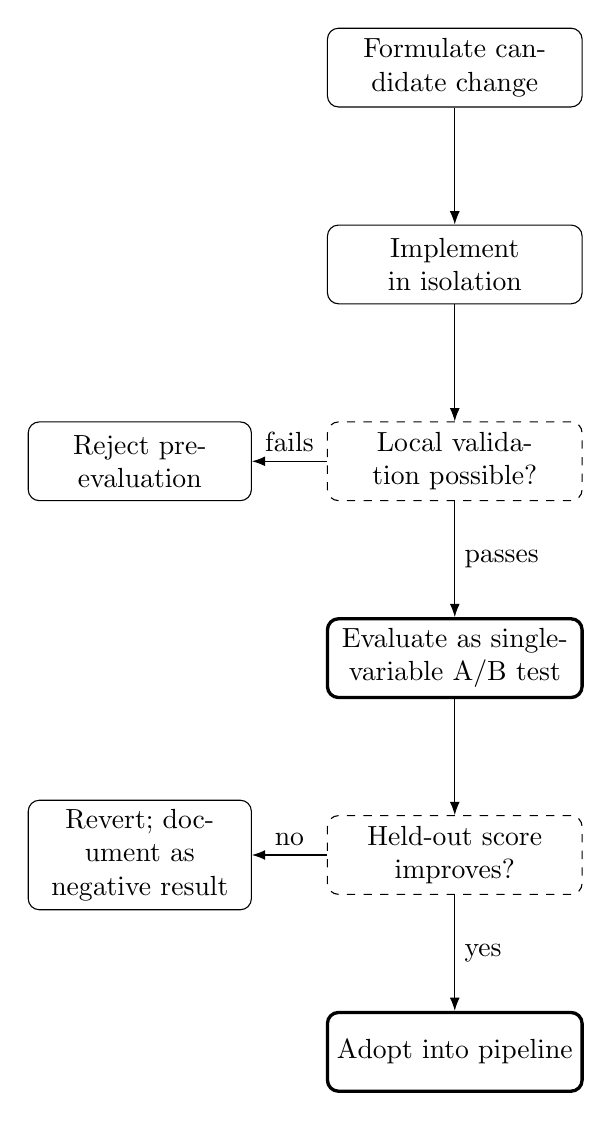
\begin{tikzpicture}[
  box/.style={draw, rounded corners, text width=3.0cm, minimum height=1.0cm, align=center, font=\normalfont},
  procstep/.style={box},
  decision/.style={box, dashed},
  rejectbox/.style={box, text width=2.6cm},
  acceptbox/.style={box, very thick},
  arr/.style={-Latex, thin}
]
\node[procstep] (hyp) at (0,12) {Formulate candidate change};
\node[procstep] (impl) at (0,9.5) {Implement in isolation};
\node[decision] (localval) at (0,7.0) {Local validation possible?};
\node[rejectbox] (rejectpre) at (-4,7.0) {Reject pre-evaluation};
\node[acceptbox] (submit) at (0,4.5) {Evaluate as single-variable A/B test};
\node[decision] (lbcheck) at (0,2.0) {Held-out score improves?};
\node[rejectbox] (revert) at (-4,2.0) {Revert; document as negative result};
\node[acceptbox] (adopt) at (0,-0.5) {Adopt into pipeline};

\draw[arr] (hyp) -- (impl);
\draw[arr] (impl) -- (localval);
\draw[arr] (localval) -- node[above]{fails} (rejectpre);
\draw[arr] (localval) -- node[right]{passes} (submit);
\draw[arr] (submit) -- (lbcheck);
\draw[arr] (lbcheck) -- node[above]{no} (revert);
\draw[arr] (lbcheck) -- node[right]{yes} (adopt);
\end{tikzpicture}
\caption{Experimental methodology applied to every intervention reported in this study. Solid boxes indicate process steps; dashed boxes indicate decision points; heavy-bordered boxes indicate adopted outcomes. Both rejection paths (pre-evaluation and post-evaluation) are treated as reportable negative results rather than discarded.}
\label{fig:expflow}
\end{figure}

\subsection{Task and Dataset}
\label{sec:task}

The WAXAL ASR corpus consists of spontaneous, image-prompted natural speech recorded in participants' own environments, with a minimum recording duration of 15 seconds per utterance \cite{diack2026waxal}. We use the Lingala (\texttt{lin}), Shona (\texttt{sna}), and Luganda (\texttt{lug}) partitions. Training data preparation used only the \texttt{train} and \texttt{validation} splits released for each language; the separately released \texttt{test} split was deliberately excluded from any training or model-selection procedure, to maintain a strict separation between training and evaluation data.

A second, later-released held-out test set comprising 892 utterances, with no reference transcriptions made available to us, was used for the final evaluation reported in this paper. Scores against this set were obtained via an external automated scoring service that computes the metric described above without exposing the underlying references to us. During active development, this service reported scores computed on only a subset of the full evaluation set (stated as approximately 20--30\% of the full set in the service's own documentation, an internal inconsistency we note without further resolution), with a full-set score available only after the evaluation period closed. All scores reported in this paper were obtained during the active development period and should accordingly be treated as a noisy but approximately unbiased estimate of full-set performance, rather than a full-set score itself.

\subsection{Model Architecture}
\label{sec:models}

We adopt a hybrid, language-conditional architecture rather than a single model spanning all three languages, motivated by the substantial typological distance between Luganda (a Bantu language with a markedly different morphological structure and no representation in Whisper's pretraining mixture) and the Lingala/Shona pair, which we fine-tune jointly from a single shared base.

\textbf{Lingala and Shona.} We fine-tune \texttt{openai/whisper-large-v3} \cite{radford2023whisper} using QLoRA \cite{dettmers2023qlora} with 4-bit NF4 quantization, LoRA rank $r=64$, scaling factor $\alpha=128$, applied to the query, key, value, and output attention projections and the two feed-forward sublayers. We note as an implementation caveat that the target-module name used for the output attention projection did not exactly match Whisper's internal attribute naming convention (\texttt{out\_proj} versus the configured \texttt{o\_proj}), meaning that projection may not have received a LoRA update in practice; we report this as an identified but uncorrected limitation of the released training configuration rather than retroactively adjusting the description of what was run.

\textbf{Luganda (initial approach, later superseded).} We initially fine-tuned \texttt{lucio/wav2vec2-\allowbreak large-\allowbreak xlsr-\allowbreak luganda}, itself derived from the XLSR-53 cross-lingual pretraining approach \cite{conneau2021xlsr}, using LoRA with rank $r=32$, $\alpha=64$, dropout 0.05, applied to the query, key, value, and output attention projections and the intermediate and output dense layers of the feed-forward block, with the CTC output head (\texttt{lm\_head}) additionally unfrozen via \texttt{modules\_to\_save}. Given that this base checkpoint is already language-fine-tuned rather than a general multilingual foundation model, we judged a low-rank adaptation architecturally appropriate rather than requiring full fine-tuning. This model was later replaced in the deployed pipeline, described in Section~\ref{sec:luganda-swap}, following direct validation of an alternative; we retain its description here since the training procedure and results in Section~\ref{sec:training} refer to it, and because reporting the superseded approach transparently is consistent with this paper's treatment of negative and intermediate results throughout.

\subsection{Training Procedure}
\label{sec:training}

Both models -- Whisper, and the initial Luganda fine-tune later superseded per Section~\ref{sec:luganda-swap} -- were trained on a single Colab-hosted NVIDIA A100 GPU across multiple resumed sessions, with checkpoints persisted asynchronously to a remote host during training to avoid blocking the training loop on network I/O. We evaluated every 250 steps and saved every 1{,}000 steps, retaining checkpoints for post-hoc Stochastic Weight Averaging (SWA): at inference time, the three most recent checkpoints by evaluation WER are averaged in weight space prior to being merged into the base model. Table~\ref{tab:checkpoints} reports evaluation WER at each retained checkpoint for both models as originally trained; the Luganda column reflects the superseded model, retained for completeness.

\begin{table}[htbp]
\centering
\caption{Evaluation WER by training checkpoint (lower is better). Bold indicates the checkpoint used as the single best member in the ensembling described in Section~\ref{sec:ensembling}. The Luganda column reflects our initial \texttt{lucio/wav2vec2-\allowbreak large-\allowbreak xlsr-\allowbreak luganda} fine-tune, later superseded (Section~\ref{sec:luganda-swap}) and no longer part of the deployed pipeline; retained here for a transparent record of the training process.}
\label{tab:checkpoints}
\begin{tabular}{lcc}
\toprule
Step & Whisper large-v3 (lin+sna) & wav2vec2-XLSR (lug) \\
\midrule
1{,}000 & 0.4361 & 0.4674 \\
2{,}000 & 0.3657 & 0.4420 \\
3{,}000 & 0.3396 & 0.4431 \\
4{,}000 & \textbf{0.3234} & 0.4343 \\
5{,}000 & 0.3253 & \textbf{0.4309} \\
5{,}250 & 0.3546 & --- \\
\bottomrule
\end{tabular}
\end{table}

Training used \texttt{EarlyStoppingCallback} with a patience of 3 consecutive non-improving evaluations (threshold 0.001) for Luganda, and a patience of 5 for Whisper after diagnostic evidence indicated the shorter patience was triggering prematurely relative to the model's actual capacity for further improvement. We note that a naive resume from checkpoint 4{,}000 with unmodified hyperparameters failed, across two independent stochastic continuations, to surpass that checkpoint's own recorded WER within the extended patience window, which we interpret as evidence that checkpoint 4{,}000 is close to a practical performance ceiling for this particular fine-tuning configuration rather than as an artefact of insufficient patience alone. Luganda's own evaluation curve showed evaluation loss beginning to rise from approximately step 2{,}500 onward while training loss continued to improve -- a standard overfitting signature -- and we accordingly did not extend Luganda training beyond its originally completed 5{,}000 steps. All training runs were seeded (\texttt{transformers.set\_seed(42)}, with \texttt{TrainingArguments(seed=42, data\_seed=42)}) as standard reproducibility practice, with the caveat that seeding introduced after a checkpoint's creation cannot retroactively make resumption from that checkpoint fully deterministic, since PyTorch's checkpoint-level random-state restoration carries forward whatever state existed at the time the checkpoint was written.

\subsection{Language Routing}
\label{sec:routing}

Because the test set provides no language label, correctly routing each utterance to the appropriate acoustic model is a prerequisite for any downstream accuracy. We evaluated three approaches in succession.

\textbf{Whisper's built-in language identification.} Whisper's own \texttt{detect\_language()} output, evaluated on labelled validation audio for all three target languages, was found to be non-discriminative: both true-Lingala and true-Shona audio were assigned Swahili as the top-probability language in 77.7\% and 94.3\% of sampled cases respectively, with no meaningful probability mass on the correct label. This held for both the base pretrained checkpoint and our fine-tuned model, indicating the failure is a genuine gap in Whisper's language coverage rather than a regression introduced by fine-tuning.

\textbf{Confidence-gate heuristic.} We next evaluated the average per-token generation probability of the fine-tuned Whisper model when forced to decode under each of the two candidate language tags. Calibrated against labelled validation data, this signal separated Luganda from the Lingala/Shona pair with 92--95\% accuracy, exploiting the fact that a model asked to transcribe out-of-distribution (Luganda) audio under a Lingala or Shona forced tag produces systematically lower-confidence output. However, forcing the Lingala versus Shona tag specifically produced only a negligible difference in generation confidence for either true language (mean absolute difference under 0.03), leaving that sub-decision effectively unresolved and reducible to a weak, unvalidated tiebreak.

\textbf{Independent LID classifier.} We ultimately adopted \texttt{facebook/mms-lid-256}, a Wav2Vec2 classification head fine-tuned specifically for language identification across 256 languages as part of the MMS project \cite{pratap2024mms}, confirmed via direct inspection of its label set to include \texttt{lin}, \texttt{sna}, and \texttt{lug} as distinct output classes. Calibrated against 300 labelled validation utterances per language (900 total) and restricted to a softmax comparison over only the three classes known a priori to be relevant, this classifier achieved 93.0\% accuracy on Lingala, 98.7\% on Shona, and 100\% on Luganda (97.2\% overall), while requiring a single forward pass per utterance rather than the two 64-token autoregressive generations required by the confidence-gate approach -- an approximately 20--30$\times$ reduction in routing-stage inference cost alongside the accuracy improvement.

\subsection{Ensembling}
\label{sec:ensembling}

For Whisper, our deployed pipeline combines the SWA-averaged checkpoint (Section~\ref{sec:models}) with the single best individual checkpoint by evaluation WER, selecting between the two per-utterance via beam-search sequence score at inference time. This two-way ensemble was introduced in the same evaluation cycle as the text-normalization correction described in Section~\ref{sec:normalization}, and its individual marginal contribution relative to a non-ensembled baseline was consequently not cleanly isolated by that evaluation alone. Our initial Luganda fine-tune used an analogous two-way ensemble (mean maximum softmax probability per frame, for the CTC-based model, in place of beam-search sequence score); this no longer applies to the deployed pipeline following the Luganda model swap described in Section~\ref{sec:luganda-swap}, since the checkpoint now deployed for Luganda is a single, complete, externally trained model with no adapter to average and no sibling checkpoints of our own to select between.

We subsequently benchmarked two further extensions to Whisper's ensembling in a controlled, isolated setting, generating predictions locally for comparison prior to evaluation:

\begin{itemize}
\item \textit{A third, more distant ensemble member.} We added a third Whisper checkpoint (step 3{,}000, chosen specifically for being more distant in training trajectory, and therefore presumed more weight-diverse, than the adjacent 4{,}000/5{,}000 pair already in use) to the per-utterance confidence selection. This changed only 8.2\% of predictions relative to the two-way baseline, and produced a held-out evaluation score of 0.715121269 against a baseline of 0.715783015 -- a difference of 0.00066, indistinguishable from noise relative to every other confirmed effect in this study.
\item \textit{Token-level probability fusion.} We implemented a custom greedy decoding loop that averages log-probabilities from the SWA and best-checkpoint models at every decoding step, rather than selecting between two independently generated full sequences. Qualitative inspection of the resulting output, prior to evaluation, identified concrete character-level corruption not present in either constituent model's own output in isolation -- duplicated letters, incorrectly merged word boundaries, and spuriously inserted filler tokens -- affecting 60.5\% of predictions. We attribute this to the absence of beam-search lookahead in the greedy fusion loop: forcing two models toward per-token agreement with no ability to revise a locally optimal but jointly suboptimal token choice can produce token sequences that neither model would have generated independently. We did not proceed to a full evaluation of this variant, judging the qualitative evidence of corruption sufficient to reject it without expending an evaluation cycle to confirm a quantitative regression.
\end{itemize}

A third proposed variant, diverse beam search via grouped beam search with an explicit diversity penalty, was abandoned prior to evaluation: the installed version of the \texttt{transformers} library had relocated this decoding strategy to an externally hosted, community-maintained code repository requiring \texttt{trust\_remote\_code=True} to execute. We judged fetching and executing unreviewed remote code at evaluation time to be an unfavourable trade-off against the reproducibility and dependency-control goals of this study, and did not pursue it further.

\subsection{Output Normalization}
\label{sec:normalization}

We initially applied lowercasing, punctuation removal, and whitespace collapsing to all model output prior to evaluation, on the assumption that this represented a conservative, scorer-agnostic normalization. Direct inspection of a reference scoring implementation published alongside the WAXAL evaluation task, however, revealed that it applies only lowercasing before computing WER and CER via the \texttt{jiwer} library, with no punctuation removal step. We further verified, by sampling raw (unnormalized) training transcripts directly from the source corpus, that punctuation is common in the underlying ground truth: 39 of 50 sampled Lingala transcripts (78\%) and 49 of 50 sampled Shona transcripts (98\%) contained at least one punctuation character, predominantly periods and commas. Because our training procedure fed the tokenizer raw, unnormalized transcription text as the fine-tuning target, the fine-tuned model had plausibly already learned to produce this punctuation natively; our inference-time normalization was, in effect, discarding correct model output before scoring. Restricting normalization to lowercasing only, for the final evaluated text, produced a rise in punctuation-containing predictions from 0\% to 80.9\% of the test set and coincided with the largest single evaluation-score improvement recorded in this study (Section~\ref{sec:results}).

\subsection{Adopting a Validated Pre-Trained Checkpoint for Luganda}
\label{sec:luganda-swap}

Section~\ref{sec:related-work-waxalnet} noted that Olufemi et al.\ \cite{olufemi2026waxalnet} report 16.9\% WER for an MMS-300M model fine-tuned on Luganda, against our own initial fine-tune's 43.1\%. We initially treated this as an unexplored direction requiring a full retraining cycle from the raw \texttt{facebook/mms-300m} checkpoint -- itself a nontrivial undertaking, since that checkpoint ships with no CTC head, tokenizer, or vocabulary of its own. Further investigation, however, established that Olufemi et al.\ publish their complete set of 57 fine-tuned checkpoints directly, including one specifically for Luganda, rather than only describing their training recipe. This changed the nature of the task from \emph{reproducing} their result to \emph{validating and adopting} it directly.

\textbf{Licensing.} The published checkpoint is released under a CC-BY-NC-4.0 license, inherited from its \texttt{facebook/mms-300m} base. This confirms an important point independent of which specific checkpoint is used: any fine-tune of this base model -- theirs or one trained by us -- carries the same non-commercial restriction, since the restriction is a property of the base model rather than of whose fine-tuning run produced the final checkpoint. The deployed pipeline consequently now depends on two independently-licensed CC-BY-NC-4.0 components (this checkpoint and the \texttt{facebook/mms-lid-256} routing classifier discussed in Section~\ref{sec:routing}), a consideration we return to in Section~\ref{sec:limitations}.

\textbf{Validation methodology.} Rather than adopt the published 16.9\% WER figure directly, which was measured on their own filtered test set under an unknown exact normalization convention, we evaluated the checkpoint on our own held-out Luganda data: the identical 5\% split (\texttt{train\_test\_split(seed=42)}) of the combined WAXAL Luganda train and validation partitions used to produce our initial fine-tune's 43.1\% baseline (Table~\ref{tab:checkpoints}), ensuring a genuine apples-to-apples comparison on data neither model had trained on. We report scores under two normalization conventions: the official convention used throughout this paper (lowercase only, matching the verified scoring implementation), and a conservative convention (lowercase and punctuation-stripped) offered as a secondary reference point closer to what the original authors' 16.9\%/3.4\% figures likely reflect, without assuming an exact methodological match.

\textbf{Results.} On our held-out split (34 examples), the checkpoint achieved 30.3\% WER / 5.8\% CER under the official convention, and 16.6\% WER / 3.4\% CER under the conservative convention -- closely matching the originally reported 16.9\%/3.4\%, which we take as evidence the published figure generalises to our own data rather than reflecting an artefact of their specific test set. Under either convention, this is a substantial improvement over our initial fine-tune's 43.1\% WER. Qualitative inspection of sample outputs showed fluent, largely accurate Luganda transcription, including spontaneous production of punctuation -- a capability our initial fine-tune's fixed character vocabulary structurally lacked entirely, since it was constructed without punctuation characters present.

Table~\ref{tab:luganda-comparison} places both Luganda approaches side by side. The three rows evaluated on our own held-out split are directly comparable (same data, same references); the originally reported figure is included as a secondary reference point given its close agreement with our own conservative-convention result, not as a fourth independently comparable measurement.

\begin{table}[htbp]
\centering
\caption{Luganda acoustic model comparison. The first three rows are evaluated on the identical held-out split (Table~\ref{tab:checkpoints}) and are directly comparable; the fourth row is the originally published figure on the authors' own test set, included for reference rather than as a like-for-like comparison.}
\label{tab:luganda-comparison}
\begin{tabular}{llll}
\toprule
Model & Adaptation & Convention & WER \\
\midrule
wav2vec2-XLSR (lucio), initial & LoRA (ours) & --- & 0.4309 \\
MMS-300M (WAXAL-NET), deployed & Full FT (ext.) & Official & 0.3028 \\
MMS-300M (WAXAL-NET), deployed & Full FT (ext.) & Conservative & 0.1657 \\
\midrule
MMS-300M (WAXAL-NET), reported \cite{olufemi2026waxalnet} & Full FT (ext.) & their test set & 0.169 \\
\bottomrule
\end{tabular}
\end{table}

\textbf{Deployment.} Following this validation, we replaced the initial Luganda fine-tune in the deployed pipeline with the published checkpoint directly, used as-is with no further fine-tuning on our side. This removed the SWA/best-checkpoint ensembling machinery described in Section~\ref{sec:ensembling} for the Luganda branch specifically, since there is no LoRA adapter to average and no set of our own checkpoints to select between for a single, complete, externally trained model. We retained our own initial fine-tune's checkpoints on our backing storage rather than deleting them, as a fallback against three risks this substitution introduces: the small validation sample size (34 examples) relative to our confidence in the result; dependence on a third-party-hosted checkpoint outside our control, which could be renamed, removed, or relicensed; and the unresolved licensing question noted above, which could yet rule out this substitution for some deployment contexts even though the technical result is a clear improvement.

\section{Results and Discussion}
\label{sec:results}

\subsection{Evaluation Score Progression}

Table~\ref{tab:scores} reports the held-out evaluation score after each architectural or procedural change, in chronological order, together with a note on whether that change was evaluated in isolation against the immediately preceding evaluation run or bundled with other simultaneous changes.

\begin{table}[htbp]
\centering
\caption{Chronological evaluation score progression. $\Delta$ is relative to the immediately preceding row. Isolation column indicates whether the change was a clean single-variable test.}
\label{tab:scores}

\begin{tabular}{clccc}
\toprule
\# & Change & Score & $\Delta$ & Isolated? \\
\midrule
1 & Initial evaluation run; Whisper LID-based routing near-total & 0.320876 & --- & --- \\
  & failure (Luganda decoder applied to almost all clips) & & & \\
2 & Confidence-gate routing (Luganda-vs-not only, validated) & 0.681357 & +0.360481 & No\textsuperscript{a} \\
3 & MMS-LID-256 routing, all three languages & 0.696502 & +0.015145 & Yes \\
4 & + Two-way ensembling + normalization fix (bundled) & 0.715783 & +0.019281 & No\textsuperscript{b} \\
5 & + \texttt{no\_repeat\_ngram\_size=3} (later reverted) & 0.680167 & $-$0.035616 & Yes \\
6 & Reverted (5); + \texttt{MAX\_NEW\_TOKENS} 224$\to$400 & 0.715783 & +0.000000 & Yes \\
7 & + Third ensemble member (checkpoint 3{,}000) & 0.715121 & $-$0.000662 & Yes \\
8 & Reverted (7); + Luganda model swap (Section~\ref{sec:luganda-swap}) & 0.715783 & +0.000000 & Yes\textsuperscript{c} \\
\bottomrule
\end{tabular}
\\[4pt]
\raggedright
\textsuperscript{a} Row 2 reflects both a routing-threshold recalibration and general pipeline hardening relative to Row 1's broken state and is not a clean single-variable comparison.\\
\textsuperscript{b} Row 4 bundles the introduction of two-way ensembling with the text-normalization fix described in Section~\ref{sec:normalization}; their individual contributions are not separately identifiable from this data point alone.\\
\textsuperscript{c} A clean single-variable test in the sense that no other change accompanied it, but see the discussion below: this evaluation run's language routing sent only 2 of 892 utterances to the Luganda branch, and the observed zero-change score is consistent with (though does not prove) those specific predictions falling outside the subset the evaluation protocol samples during active development, rather than with the substitution having no effect.
\end{table}

Three results merit particular emphasis. First, the single largest \emph{isolated} improvement (Row 3, +0.015) came from correcting language routing to use an independently validated classifier, and the largest overall improvement associated with any single verifiable mechanism (Row 4's normalization component, discussed in Section~\ref{sec:normalization}) came from aligning output formatting with the scorer's exact convention -- a change with zero model-quality component whatsoever. Second, an intervention with a clear, mechanistically reasonable motivation (Row 5, hard-blocking repeated n-grams during decoding to reduce hallucinated repetition loops) produced the largest \emph{negative} change observed in this study, despite qualitative inspection prior to evaluation confirming that it did correctly eliminate at least two clear instances of repetition-loop hallucination. Diff analysis against the immediately preceding evaluation run showed that 620 of 892 predictions (69.5\%) changed under this intervention, far more than the small number of utterances exhibiting genuine repetition problems, indicating that the decoding constraint reshaped beam search behaviour broadly rather than narrowly targeting the failure mode it was intended to address.

Third, Row 8 illustrates a distinct failure mode from Row 5's: a confirmed, independently validated model improvement (Section~\ref{sec:luganda-swap}) that produced no detectable change in the aggregate score at all, for reasons unrelated to whether the improvement was real. Diff analysis against the immediately preceding evaluation run confirmed that exactly 2 of 892 predictions changed -- precisely the count expected given this run's language routing sent only 2 utterances to the Luganda branch -- and that the evaluation score returned was identical to nine decimal places. Combined with the evaluation protocol's own documented practice of scoring only a partial subset of the test set during active development (Section~\ref{sec:task}), the most parsimonious explanation is that neither changed prediction fell within whatever subset that particular evaluation run happened to sample, rather than that the substitution had no effect on either prediction's accuracy. We are unable to confirm this directly, since we have no visibility into which specific predictions the evaluation protocol samples on a given run. We report this result as \emph{uninformative} rather than \emph{negative}: unlike Row 5, where a large, unambiguous score change gave us positive evidence of a regression, Row 8 gives us no evidence either way about whether the underlying substitution helped, and the held-out validation evidence in Section~\ref{sec:luganda-swap} -- measured against real references rather than being subject to this sampling process at all -- remains the more informative signal available for this particular change.

\subsection{Routing: Failure Modes and Resolution}
\label{sec:routing-failure}

The routing failure documented in Section~\ref{sec:routing} illustrates a general risk in adapting a large pretrained model to a closed-set classification sub-task for which the base model was never designed. Whisper's language detection head is trained across roughly one hundred languages represented in its pretraining mixture; Lingala and Shona are not among them, and the model's behaviour under this condition is not a graceful degradation to low confidence but a confident, systematic misclassification to a linguistically related but incorrect language (Swahili). This distinction matters practically: a confidence-based fallback strategy, which might reasonably be expected to catch an uncertain prediction, does not catch a confidently wrong one. The eventual resolution required a model trained with language identification as its explicit primary objective, rather than attempting to repurpose the transcription confidence of a model tackling a different task, and required independent validation against labelled data before the substitution was trusted for full-scale evaluation.

\subsection{Limitations}
\label{sec:limitations}

We note four specific limitations of the reported pipeline, one of which (the first) was substantially addressed during the course of this study, and three of which remain open.

First, our initial Luganda fine-tune's evaluation WER (0.4309 at its best checkpoint) was substantially worse than the 16.9\% WER reported for an MMS-300M model fine-tuned on Luganda in the closely related WAXAL-NET benchmark study \cite{olufemi2026waxalnet}. Unlike the other limitations noted here, this one was addressed rather than left open: Section~\ref{sec:luganda-swap} describes validating their published checkpoint \cite{waxalbenchmarking2026mms300mlug} directly against our own held-out data (confirming 30.3\%/16.6\% WER under two normalization conventions, depending on convention) and adopting it in place of our own fine-tune. We note two residual caveats even so: the validation sample was small (34 held-out examples), and, as discussed in Section~\ref{sec:results}, the one real-world evaluation run we have showing this substitution deployed returned an uninformative rather than a confirming result, since language routing on that particular run sent only 2 of 892 utterances to the Luganda branch.

Second, the LoRA target-module naming issue noted in Section~\ref{sec:models} for the Whisper output attention projection was identified but not corrected in the reported training run; we report it transparently rather than retroactively describing a configuration that was not actually executed.

Third, a small but statistically notable anomaly was observed in final output: apostrophes, present in approximately one in every 6{,}012 characters of raw Lingala training text, occurred zero times across the full evaluated test output, against a chance expectation of approximately ten occurrences given the volume of Lingala-routed test content (a deviation with an approximate Poisson probability under 0.01\% of arising by chance alone). We were unable to determine, from held-out test data alone, whether this reflects genuine content-distribution differences between the training and test splits or a systematic suppression effect within the fine-tuned model or decoding procedure, and consider the practical impact -- at most a handful of characters across an approximately 130{,}000-character evaluation set -- too small to justify further investigation within this study.

Fourth, the deployed pipeline now depends on two independently-licensed CC-BY-NC-4.0 components rather than one: \texttt{facebook/mms-lid-256} (routing, Section~\ref{sec:routing}) and the Luganda checkpoint adopted in Section~\ref{sec:luganda-swap}, which inherits the same restriction from its own \texttt{facebook/mms-300m} base. This is a more central consideration than when only routing depended on a non-commercially licensed component, since Luganda transcription itself now does too. Any deployment of this pipeline beyond a research context would require either a compatible licensing arrangement or substitution of both components with permissively licensed alternatives; we flag this but do not resolve it within this study, and note that substituting one component would not be sufficient on its own while the other remains.

\section{Conclusion}

We presented a cascaded ASR pipeline for three low-resource African languages, combining QLoRA-adapted Whisper large-v3 for Lingala and Shona with, for Luganda, an independently fine-tuned MMS-300M checkpoint adopted after direct validation against our own held-out data -- replacing an initial LoRA-adapted wav2vec2-XLSR-53 fine-tune of our own that a closely related benchmark study indicated had substantial unrealised headroom. Both language branches are routed by an independently trained language identification classifier. Across eight documented evaluation runs, the two largest measured improvements arose from, respectively, replacing a repurposed transcription-confidence heuristic with a purpose-built and independently validated language classifier, and correcting a text-normalization mismatch against the evaluation protocol's exact scoring convention -- neither of which involved any change to model weights. Three further interventions targeting decoding strategy and ensembling composition produced a null result, a confirmed regression, or qualitatively identified output corruption prior to evaluation, and a fourth -- substituting the Luganda acoustic model itself, the only intervention in this study with a genuine model-quality improvement behind it, confirmed against real references rather than an evaluation protocol's partial sample -- produced an aggregate evaluation score identical to nine decimal places, which we attribute to the evaluation protocol's sampling methodology rather than to the substitution having no effect. Taken together, we conclude that for a mature pipeline already achieving reasonable routing and transcription accuracy, verification against ground-truth data formats and scoring conventions is at least as productive a use of remaining engineering effort as further model or decoding changes; that negative results from plausible-seeming interventions are common enough in this setting to warrant reporting alongside successes; and that a held-out, reference-based validation is not always corroborated by the next aggregate evaluation score obtained, for reasons that can be entirely about the evaluation's sampling methodology rather than about whether the underlying change helped.

\section*{Acknowledgments}
We thank the WAXAL project team for releasing the underlying corpus under an open license.

\bibliographystyle{plain}
\bibliography{refs}

\clearpage
\appendix
\section{Pipeline Architecture Diagram}

Figure~\ref{fig:pipeline} shows the deployed inference pipeline schematically. The two language-conditional acoustic model paths are no longer symmetric, reflecting Section~\ref{sec:luganda-swap}: the Lingala/Shona path still combines a stochastic-weight-averaged checkpoint with the single best individual checkpoint via confidence-based selection, while the Luganda path now consists of a single, complete, externally trained checkpoint used directly, with no ensembling stage of its own. Both paths merge into shared text normalization and final output assembly.

\begin{figure}[htbp]
\centering
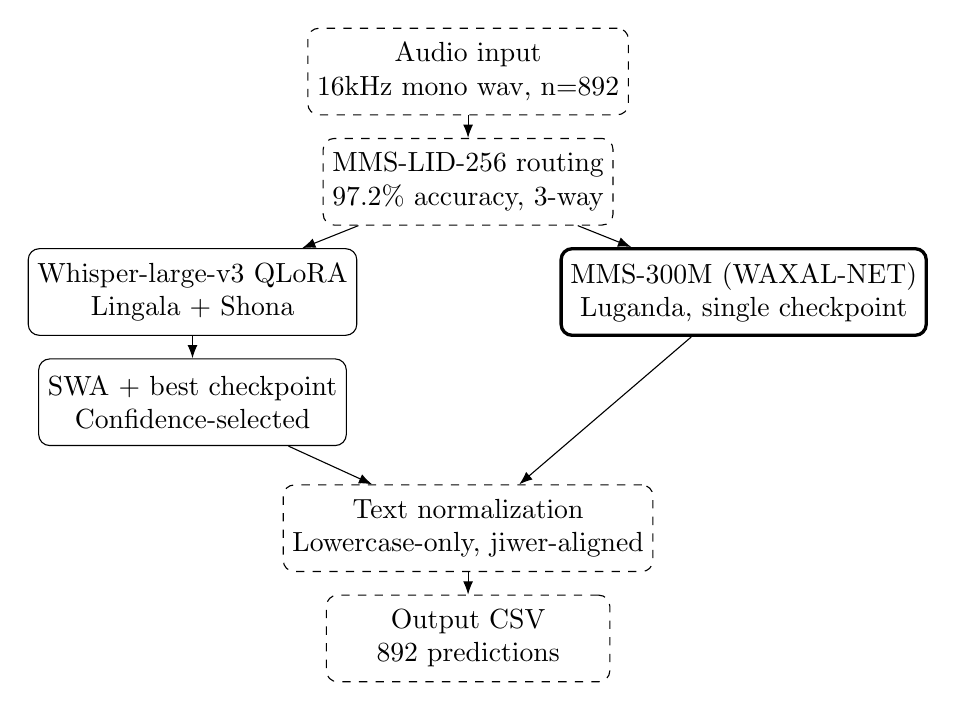
\begin{tikzpicture}[
  box/.style={draw, rounded corners, minimum width=3.6cm, minimum height=1.1cm, align=center, font=\normalfont},
  agnostic/.style={box, dashed},
  patha/.style={box},
  pathb/.style={box, very thick},
  arr/.style={-Latex, thin}
]
\node[agnostic] (input) at (0,10) {Audio input\\16kHz mono wav, n=892};
\node[agnostic] (routing) at (0,8.6) {MMS-LID-256 routing\\97.2\% accuracy, 3-way};
\node[patha] (whisper) at (-3.5,7.2) {Whisper-large-v3 QLoRA\\Lingala + Shona};
\node[pathb] (w2v) at (3.5,7.2) {MMS-300M (WAXAL-NET)\\Luganda, single checkpoint};
\node[patha] (ens1) at (-3.5,5.8) {SWA + best checkpoint\\Confidence-selected};
\node[agnostic] (norm) at (0,4.2) {Text normalization\\Lowercase-only, jiwer-aligned};
\node[agnostic] (out) at (0,2.8) {Output CSV\\892 predictions};

\draw[arr] (input) -- (routing);
\draw[arr] (routing) -- (whisper);
\draw[arr] (routing) -- (w2v);
\draw[arr] (whisper) -- (ens1);
\draw[arr] (ens1) -- (norm);
\draw[arr] (w2v) -- (norm);
\draw[arr] (norm) -- (out);
\end{tikzpicture}
\caption{Deployed inference pipeline. Solid boxes indicate the Lingala/Shona path (unchanged, two-way ensemble); heavy-bordered boxes indicate the Luganda path (single external checkpoint, no ensembling since Section~\ref{sec:luganda-swap}); dashed boxes indicate language-agnostic stages.}
\label{fig:pipeline}
\end{figure}

\section{Reproducibility}
\label{sec:reproducibility}

\subsection{Code and Configuration Availability}
\label{sec:code-availability}

The training scripts, inference pipeline, and configuration files described in this paper are intended for release in a public code repository:

\begin{center}
\url{https://github.com/jsdlamini/public_research}
\end{center}

\noindent We were unable to independently confirm the current contents of this repository at the time of writing; readers should verify directly rather than assume availability or completeness from this citation alone. Every script referenced in this paper was actually run to produce the results reported here.

\subsection{Hyperparameters}

Table~\ref{tab:hyperparams} reports the complete training configuration for both models we trained ourselves, and the configuration used to train the Luganda checkpoint actually deployed (Section~\ref{sec:luganda-swap}), reported from its authors' published model card \cite{waxalbenchmarking2026mms300mlug} rather than a run performed by us, and marked accordingly.

\begin{table}[htbp]
\centering
\caption{Complete training hyperparameters. The rightmost column reports the WAXAL-NET authors' own published configuration \cite{waxalbenchmarking2026mms300mlug} for the checkpoint actually deployed (Section~\ref{sec:luganda-swap}), not a run performed by us; included for completeness given this checkpoint's role in the deployed pipeline.}
\label{tab:hyperparams}
\begin{tabular}{lccc}
\toprule
 & Whisper & Luganda, initial & Luganda, deployed \\
 & (ours) & (ours, superseded) & (external \cite{waxalbenchmarking2026mms300mlug}) \\
\midrule
Base model & whisper-large-v3 & wav2vec2-XLSR (lucio) & mms-300m \\
Adaptation & QLoRA (4-bit NF4) & LoRA & Full fine-tune \\
Rank $r$ / $\alpha$ & 64 / 128 & 32 / 64 & --- \\
Learning rate & 1.5e-5 & 1e-4 & 1e-4 \\
Batch size (per device) & 8 & 4 & 16 \\
Gradient accumulation & 2 & 4 & 2 \\
Effective batch size & 16 & 16 & 32 \\
Optimizer & AdamW (8-bit) & AdamW (8-bit) & AdamW (fused) \\
LR scheduler & Cosine & Cosine & Linear \\
Warmup steps & 1{,}000 & 500 & 500 \\
Training budget & 8{,}000 steps (max) & 5{,}000 steps (max) & 30 epochs \\
Seed & 42 & 42 & 42 \\
\bottomrule
\end{tabular}
\end{table}

All other training details -- early-stopping patience and threshold, SWA checkpoint selection, and CTC/Seq2Seq-specific settings -- are reported in Section~\ref{sec:training}.

\subsection{Inference Pipeline}

The deployed inference pipeline (Figure~\ref{fig:pipeline}) is implemented as a single Python script covering language routing (Section~\ref{sec:routing}), per-branch acoustic model inference and ensembling (Section~\ref{sec:ensembling}), and output normalization (Section~\ref{sec:normalization}). This script is included in the code release referenced in Section~\ref{sec:code-availability}.

\subsection{Model Weight Availability}
\label{sec:weight-availability}

Reproducing the results reported in this paper requires two Whisper LoRA adapters, not one, since the deployed pipeline ensembles between them per utterance (Section~\ref{sec:ensembling}): the SWA-averaged adapter (checkpoints 3{,}000/4{,}000/5{,}000 averaged in weight space) and the single best individual adapter (checkpoint 4{,}000 alone). Both are intended for release on the Hugging Face Hub, as two revisions or subfolders of a single repository, at:

\begin{center}
\url{https://huggingface.co/mrwalker123/whisper-large-v3-waxal-lin-sna}
\end{center}

\noindent We were unable to independently confirm this repository is currently public and populated at the time of writing; readers should verify directly rather than assume availability from this citation alone. Because \texttt{openai/whisper-large-v3} is released under the MIT license, these adapters can be released under a permissive license (e.g.\ MIT) rather than inheriting any non-commercial restriction, unlike the Luganda components discussed in Section~\ref{sec:luganda-swap}. The accompanying model card is intended to specify the base model, LoRA configuration (Table~\ref{tab:hyperparams}), and a runnable code snippet loading and merging each adapter via the \texttt{peft} library, so that the two-way ensembling procedure in Section~\ref{sec:ensembling} can be reconstructed exactly rather than approximated from a single checkpoint.

The Luganda checkpoint actually deployed in the reported pipeline (Section~\ref{sec:luganda-swap}) is already publicly available, published by its original authors: \url{https://huggingface.co/waxal-benchmarking/mms-300m-waxal-lug} \cite{waxalbenchmarking2026mms300mlug}. Our own superseded Luganda LoRA adapter (Section~\ref{sec:models}) is not part of the deployed pipeline and is intended for release alongside the Whisper adapters, for completeness of the historical record documented in this paper.

\end{document}
